\section{Problem 5-1 Configuration Model}



\begin{enumerate}
	\item \textbf{1.} Such a network cannot exist. The first node has a degree of 4.  In the remaining network (without this node), only 2 stubs exist (node 2: 1 and node 3:1).  This means there are not enough stubs to connect the stubs of node 1 to,  without creating self-loops.
	
	\item \textbf{2. } The network can exist.
	\begin{figure}[h]
		\centering
		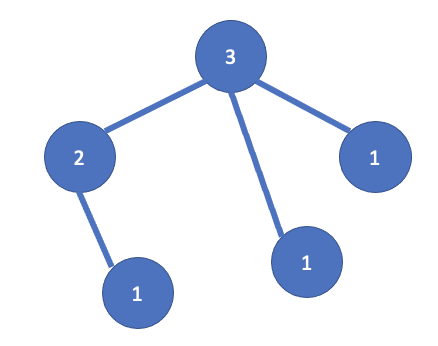
\includegraphics[width=0.9\linewidth]{images/pic1.png}
		\caption{Example Network}
		\label{distribution}
	\end{figure}
	
	\item \textbf{3.} Such a network cannot exits.  If the connections for the first node with degree 3 are fulfilled,  there are only two stubs remaining.  Since this first node has to connect to all other nodes to obtain three connections,  the remaining stubs can only be of the second node with degree 3.  To achieve the degree of 3 for this node,  the two remaining stubs would have to be connected to each other,  creating a self-loop,  which is not allowed.
\end{enumerate}